\documentclass[12pt]{article}


 \usepackage[siunitx, RPvoltages]{circuitikz}

\begin{document}


\tikz \draw (0,0) to[R=$R_1$] (2,0);


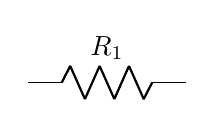
\begin{tikzpicture}
\draw (0,0) to[R=$R_1$] (2,0);
\end{tikzpicture}



\begin{circuitikz}[american]
 \draw (0,0) to[isource, l=$I_0$] (0,3) --(2,3)
 to[R=$R_1$] (2,0) -- (0,0);
 \draw (2,3) -- (4,3) to[R=$R_2$]
 (4,0) -- (2,0);
\end{circuitikz}




\begin{circuitikz}[american]
 \draw (0,0) to[isource, l=$I_0$] (0,3);
 \draw (0,3) -- (2,3) ;
 \draw (2,3) to[R=$R_1$] (2,0);
 \draw (2,0) -- (0,0);
 \draw (2,3) -- (4,3);
 \draw (4,3) to[R=$R_2$] (4,0);
 \draw  (4,0) -- (2,0);
\end{circuitikz}






\begin{circuitikz}[american]
 \draw (0,0) to[isource, l=$I_0$] (0,3)
 to[short, -*, i=$I_0$] (2,3)
 to[R=$R_1$, i=$i_1$] (2,0) -- (0,0);
 \draw (2,3) -- (4,3)
 to[R=$R_2$, i=$i_2$]
 (4,0) to[short, -*] (2,0);
\end{circuitikz}







\begin{circuitikz}[american]
 \draw (0,0) to[isource, l=$I_0$] (0,3)
 to[short, -*, i=$I_0$] (2,3)
 to[R=$R_1$, i>_=$i_1$] (2,0) -- (0,0);
 \draw (2,3) -- (4,3)
 to[R=$R_2$, i>_=$i_2$]
 (4,0) to[short, -*] (2,0);
\end{circuitikz}







\begin{circuitikz}[american, voltage shift=0.5]
 \draw (0,0) to[isource, l=$I_0$, v=$V_0$] (0,3)
 to[short, -*, i=$I_0$] (2,3)
 to[R=$R_1$, i>_=$i_1$] (2,0) -- (0,0);
 \draw (2,3) -- (4,3)
 to[R=$R_2$, i>_=$i_2$]
 (4,0) to[short, -*] (2,0);
\end{circuitikz}








\begin{circuitikz}[european, voltage shift=0.5]
 \draw (0,0) to[isourceC, l=$I_0$, v=$V
_0$] (0,3)
 to[short, -*, f=$I_0$] (2,3)
 to[R=$R_1$, f>_=$i_1$] (2,0) -- (0,0);
 \draw (2,3) -- (4,3)
 to[R=$R_2$, f>_=$i_2$]
 (4,0) to[short, -*] (2,0);
\end{circuitikz}








\begin{circuitikz}[american, voltage shift
=0.5]
 \draw (0,0) to[isource, l=$I_0$, v=$V_0$]
(0,3)
 to[short, -*, f=$I_0$] (2,3)
 to[R=$R_1$, f>_=$i_1$] (2,0) -- (0,0);
 \draw (2,3) -- (4,3)
 to[R=$R_2$, f>_=$i_2$]
 (4,0) to[short, -*] (2,0);
 \draw[red, thick] (1.5,2.5) rectangle
(4.5,3.5)
 node[pos=0.5, above]{KCL};
\end{circuitikz}


\def\coord(#1){coordinate(#1)}
\def\coord(#1){node[circle, red, draw, inner sep=1pt,pin={[red, overlay, inner
sep=0.5pt, font=\tiny, pin distance=0.1cm, pin edge={red, overlay
,}]45:#1}](#1){}}



\begin{circuitikz}[american,]
 \draw (0,0) node[npn](Q){};
 \path (Q.center) \coord(center)
 (Q.B) \coord(B) (Q.C) \coord(C)
 (Q.E) \coord(E);
\end{circuitikz}



\begin{circuitikz}[american,]
 \ctikzset{tripoles/mos style/arrows}
 \def\killdepth#1{{\raisebox{0pt}[\height][0pt]{#1}}}
 \draw (0,0) node[nmos](Q1){};
 \draw (Q1.center) node[right]{\killdepth{Q1}};
\end{circuitikz}






\def\killdepth#1{{\raisebox{0pt}[\height][0pt]{#1}}}






\begin{circuitikz}[american,]
 \draw (0,0) node[nmos,](Q1){};
 \draw (Q1.center) node[right]{\killdepth{Q1}};
 \draw (Q1.S) to[R, l2^=$R_S$ and \SI{5}{k\ohm}]
++(0,-3)
 node[vee](VEE){$V_{EE}=\SI{-10}{V}$};
 \draw (Q1.D) to[R, l2_=$R_D$ and \SI{10}{k\ohm}]
++(0,3)
 node[vcc](VCC){$V_{CC}=\SI{10}{V}$};
 \draw (Q1.S) to[short] ++(2,0) to[C=$C_1$]
++(0,-1.5) node[ground](GND){};
 \path (GND) \coord(GND) (VCC) \coord(VCC)
 (VEE) \coord(VEE);
\end{circuitikz}


\newpage









\begin{circuitikz}[
 bigR/.style={R, resistors/scale=1.8}
 ]
 \draw (0,3) to [bigR, o-o] ++(4,0);
 \draw (0,1.5) to [bigR, o-o] ++(4,0)
 to[R, o-o] ++(2,0); % ok now
 \draw (0,0) to [R, o-o] ++(4,0);
\end{circuitikz}








{
\ctikzset{bipoles/thickness=1}
\tikz \draw (0,0) to[C=1<\farad>] (2,0); \par
\ctikzset{bipoles/thickness=4}
\tikz \draw (0,0) to[C=1<\farad>] (2,0); \par

\tikz \draw (0,0) to[R=1<\ohm>] (2,0); \par
\ctikzset{bipoles/resistor/height=.6}
\tikz \draw (0,0) to[R=1<\ohm>] (2,0);
}











\def\killdepth#1{{\raisebox{0pt}[\height][0pt]{#1}}}
 \newcommand\bjtname[1]{($(#1.C)!0.5!(#1.E)$) node[anchor=west]{\killdepth{#1}} }
 \begin{circuitikz}[american, cute inductors]
 \node [op amp](A1){\texttt{OA1}};
 \draw (A1.-) to[short] ++(0,1) coordinate(tmp) to[R, l_=$R$] (tmp -| A1.out) to[short] (A1.out);
 \draw (tmp) to[short] ++(0,1) coordinate(tmp) to[C=$C$] (tmp -| A1.out) to[short] (A1.out);
 \draw (A1.+) to [battery2, invert] ++(0,-2.5) node[ground](GND){};
 \draw (A1.-) to [L=$L$] ++(-2,0) coordinate(tmp) to[sV, l=$v_s$, fill=yellow] (tmp |-GND) node[ground]{};
 \draw (A1.out) to[R=$R_s$] ++(2,0) coordinate(bb) to[I, l_=$I_B$, invert] ++(0,2) node[vcc](VCC){};
 \draw (bb) to[D, l=$D$, *-] ++(0,-2) coordinate(bb1) to[R=$R_m$] ++(0,-2) node[vee](VEE){};
 \draw (bb) --++(1,0) node[npn, anchor=B](Q1){} \bjtname{Q1};
 \draw (bb1) --++(1,0) node[pnp, anchor=B](Q2){} \bjtname{Q2};
 \draw (Q1.E) -- (Q2.E) ($(Q1.E)!0.5!(Q2.E)$) to [short, *-o, name=S] ++(2.5,0)
 node[right]{$v_{o_Q}$};
 \draw (S.s) to[european resistor, l=$Z_L$, *-] (S.s|-GND) node[ground]{};
 \draw (Q1.C) -- (Q1.C|-VCC) node[vcc]{\SI{5}{V}};
 \draw (Q2.C) -- (Q2.C|-VEE) node[vee]{\SI{-5}{V}};
\end{circuitikz}















\begin{circuitikz}[american, cute inductors]

\ctikzset{resistors/scale=0.8, % smaller R
 capacitors/scale=0.7, % even smaller C
 diodes/scale=0.6, % small diodes
 transistors/scale=1.3 } % bigger BJTs

\ctikzset{
 amplifiers/fill=cyan,
 sources/fill=green,
 diodes/fill=red,
 resistors/fill=violet,
}

 \node [op amp](A1){\texttt{OA1}};
 \draw (A1.-) to[short] ++(0,1) coordinate(tmp) to[R, l_=$R$] (tmp -| A1.out) to[short] (A1.out);
 \draw (tmp) to[short] ++(0,1) coordinate(tmp) to[C=$C$] (tmp -| A1.out) to[short] (A1.out);
 \draw (A1.+) to [battery2, invert] ++(0,-2.5) node[ground](GND){};
 \draw (A1.-) to [L=$L$] ++(-2,0) coordinate(tmp) to[sV, l=$v_s$, fill=yellow] (tmp |-GND) node[ground]{};
 \draw (A1.out) to[R=$R_s$] ++(2,0) coordinate(bb) to[I, l_=$I_B$, invert] ++(0,2) node[vcc](VCC){};
 \draw (bb) to[D, l=$D$, *-] ++(0,-2) coordinate(bb1) to[R=$R_m$] ++(0,-2) node[vee](VEE){};
 \draw (bb) --++(1,0) node[npn, anchor=B](Q1){} \bjtname{Q1};
 \draw (bb1) --++(1,0) node[pnp, anchor=B](Q2){} \bjtname{Q2};
 \draw (Q1.E) -- (Q2.E) ($(Q1.E)!0.5!(Q2.E)$) to [short, *-o, name=S] ++(2.5,0)
 node[right]{$v_{o_Q}$};
 \draw (S.s) to[european resistor, l=$Z_L$, *-] (S.s|-GND) node[ground]{};
 \draw (Q1.C) -- (Q1.C|-VCC) node[vcc]{\SI{5}{V}};
 \draw (Q2.C) -- (Q2.C|-VEE) node[vee]{\SI{-5}{V}};
\end{circuitikz}











\begin{circuitikz}
 \draw(0,0) to [nV, l=$e_n$] ++(2,0);
 \draw(0,-2) to [nI, l=$i_n$] ++(2,0);
 \begin{scope}[circuitikz/bipoles/noise
sources/fillcolor=red!50]
 \draw(3,0) to [nV, l=$e_n$] ++(2,0);
 \draw(3,-2) to [nI, l=$i_n$] ++(2,0);
 \end{scope}
 \begin{scope}[circuitikz/bipoles/noise
sources/fillcolor=green!50]
 \draw(6,0) to [nV, l=$e_n$] ++(2,0);
 \draw(6,-2) to [nI, l=$i_n$] ++(2,0);
 \end{scope}
\end{circuitikz}









\begin{circuitikz}
 \draw(0,0) to [nV, l=$e_n$] ++(2,0);
 \draw(0,-2) to [nI, l=$i_n$] ++(2,0);
 \begin{scope}[circuitikz/bipoles/noise
sources/fillcolor=dashed]
 \draw(3,0) to [nV, l=$e_n$] ++(2,0);
 \draw(3,-2) to [nI, l=$i_n$] ++(2,0);
 \end{scope}
\end{circuitikz}







\begin{circuitikz}
 \ctikzset{bipoles/noise sources/fillcolor=
dashed}
 \draw(0,0) to [nV, l=$e_n$] ++(2,0);
 \draw(0,-2) to [nI, l=$i_n$] ++(2,0);
 \begin{scope}
 \draw(3,0) to [nV, l=$e_n$, fill=yellow!50!red] ++(2,0);
 \draw(3,-2) to [nI, l=$i_n$, fill=blue!50!white] ++(2,0);
 \end{scope}
\end{circuitikz}










\begin{circuitikz}
 \draw (0,0) -- ++(1,0) to[R] ++(2,0)
 to [ammeter] ++(0,-2) node[ground]{};
 \draw (1,0) to[voltmeter] ++(0,-2)
 node[ground]{};
\end{circuitikz}













\begin{circuitikz}[american]
 \draw (0,0) -- ++(1,0) to[R] ++(2,0)
 to [rmeterwa, t=A, i=$i$] ++(0,-2) node[ground]{};
 \draw (1,0) to[rmeterwa, t=V, v=$v$] ++(0,-2)
 node[ground]{};
\end{circuitikz}







\begin{circuitikz}[]
 \draw(1,-1) to[short] (1,1)
 (0,0) to[short] (2,0);
 \draw(4,-1) to[short] (4,1)
 (3,0) to[short] (5,0)
 (4,0) node[circ]{};
\end{circuitikz}








\begin{circuitikz}[]
 \draw(1,-1) to[short] (1,1) (0,0) to[crossing]
(2,0);
 \draw(4,-1) to[short] (4,1) (3,0) to[short]
(5,0)
 (4,0) node[circ]{};
\end{circuitikz}









\begin{circuitikz} \draw
 (0,0) node[nmos] (mos) {}
 (mos.gate) node[anchor=east] {G}
 (mos.drain) node[anchor=south] {D}
 (mos.source) node[anchor=north] {S};
\end{circuitikz}










\begin{circuitikz} \draw
 (0,0) node[pigfete] (pigfete) {}
 (pigfete.G) node[anchor=east] {G}
 (pigfete.D) node[anchor=north] {D}
 (pigfete.S) node[anchor=south] {S}
 (pigfete.bulk) node[anchor=west] {Bulk};
\end{circuitikz}












\begin{circuitikz} \draw
 (0,0) node[pjfet] (pjfet) {}
 (pjfet.G) node[anchor=east] {G}
 (pjfet.D) node[anchor=north] {D}
 (pjfet.S) node[anchor=south] {S};
\end{circuitikz}










\begin{circuitikz} \draw
 (0,0) node[npn] (npn) {}
 (npn.base) node[anchor=east] {B}
 (npn.collector) node[anchor=south] {C}
 (npn.emitter) node[anchor=north] {E};
\end{circuitikz}











\begin{circuitikz} \draw
 (0,0) node[pigbt] (pigbt) {}
 (pigbt.B) node[anchor=east] {B}
 (pigbt.C) node[anchor=north] {C}
 (pigbt.E) node[anchor=south] {E};
\end{circuitikz}













\begin{circuitikz} \draw
 (0,0) node[pnp] (pnp2) {2}
 (pnp2.B) node[pnp, xscale=-1, anchor=B] (pnp1) {}
 (pnp1) node {1}
 (pnp1.C) node[npn, anchor=C] (npn1) {}
 (pnp2.C) node[npn, xscale=-1, anchor=C] (npn2) {}
 (pnp1.E) -- (pnp2.E) (npn1.E) -- (npn2.E)
 (pnp1.B) node[circ] {} |- (pnp2.C) node[circ] {};
\end{circuitikz}






\begin{circuitikz} \draw[yscale=1.1, xscale=.8]
 (2,4.5) -- (0,4.5) to[Tpmos, n=p1] (0,3)
 to[Tnmos, n=n1] (0,1.5)
 to[Tnmos, n=n2] (0,0) node[ground] {}
 (2,4.5) to[Tpmos,n=p2] (2,3) to[short, -*] (0,3)
 (p1.G) -- (n1.G) to[short, *-o] ($(n1.G)+(3,0)$)
 (n2.G) ++(2,0) node[circ] {} -| (p2.G)
 (n2.G) to[short, -o] ($(n2.G)+(3,0)$)
 (0,3) to[short, -o] (-1,3);
\end{circuitikz}










\begin{circuitikz}
 \draw (0,0) node[ground](GND){} to [sV] ++(0,2) -- ++(1,0)
 node[transformer, circuitikz/inductors/coils=6,
 anchor=A1](T){};
 \draw (T.A2) to[short, -*] (T.A2-|GND);
 \draw (T-L2.midtap) to[short, *-o] (T.B1 |- T-L2.midtap);
 \node [ocirc] at (T.B1){}; \node [ocirc] at (T.B2){};
\end{circuitikz}












\begin{circuitikz}
 \ctikzset{transformer L1/.style={inductors/width=1.8,
inductors/coils=13}}
 % too small!
 \draw (0,0) node[transformer core](T1){};
 % adjust it
 \ctikzset{quadpoles/transformer core/height=2.4}
 \draw (2.5,0) node[transformer core](T1){};
\end{circuitikz}








\begin{circuitikz}
 \draw (0,3) node[american and port] (A) {P1};
 \begin{scope}
 \ctikzset{tripoles/american or port/height=1.6}
 \draw (A.out) -- ++(0.5,0)
 node[american or port,
 number inputs=5,
 anchor=in 1] (B) {P2};
 \end{scope}
 \draw (0,1.5) node[american or port] (C) {P3};
 \draw (C.out) |- (B.in 2);
\end{circuitikz}









\begin{circuitikz}
 \draw (0,3) node[american and port] (A) {P1};
 \node at (A.bin 1) [ocirc, left]{} ;
 \begin{scope}
 \ctikzset{tripoles/american or port/height=1.6}
 \draw (A.out) -- ++(0.5,0) node[american or port,
 number inputs=5, anchor=in 1] (B) {P2};
 \node at (B.bin 3) [ocirc, left]{} ;
 \end{scope}
 \draw (0,1.5) node[american or port] (C) {P3};
 \node at (C.bin 2) [ocirc, left]{} ;
 \draw (C.out) |- (B.in 2);
\end{circuitikz}











\begin{circuitikz} \draw
 (0,2) node[and port] (myand1) {}
 (0,0) node[and port] (myand2) {}
 (2,1) node[xnor port] (myxnor) {}
 (myand1.out) -| (myxnor.in 1)
 (myand2.out) -| (myxnor.in 2);
\end{circuitikz}





\begin{circuitikz} \draw
 (0,2) node[and port] (myand1) {}
 (0,0) node[and port] (myand2) {}
 (2,1) node[xnor port] (myxnor) {}
 (myand1.out) -| (myxnor.in 1)
 (myand2.out) -| (myxnor.in 2);
\end{circuitikz}













\begin{circuitikz} \draw
 (1,0) node[not port] (not1) {}
 (3,0) node[not port] (not2) {}
 (0,0) -- (not1.in)
 (not2.in) -- (not1.out)
 ++(0,-1) node[ground] {} to[C] (not1.out)
 (not2.out) -| (4,1) -| (0,0);
\end{circuitikz}














\begin{circuitikz}
 \ctikzset{multipoles/thickness=4}
 \ctikzset{multipoles/external pins thickness=2}
 \draw (0,0) node[dipchip,
 num pins=12,
 hide numbers,
 external pins width=0.3,
 external pad fraction=4 ](C){IC1};
 \draw (C.pin 1) -- ++(-0.5,0) to[R]
 ++(0,-3) node[ground]{};
 \node [right, font=\tiny]
 at (C.bpin 1) {RST};
\end{circuitikz}
















\begin{circuitikz}
 \draw (0,0) node[dipchip,
 num pins=8,
 external pins width=0.0](C){IC1};
 \draw (C.pin 1) -- ++(-0.5,0) to[R]
 ++(0,-1.5) node[ground]{};
\end{circuitikz}














\begin{circuitikz}
 \ctikzset{multipoles/font={\color{red}\tiny}}
 \draw (0,0) node[qfpchip,
 num pins=16,
 external pad fraction=6](C){IC1};
 \draw (C.pin 1) -- ++(-0.5,0) to[R]
 ++(0,-2) node[ground]{};
\end{circuitikz}



















\begin{circuitikz}
 \draw (0,0) node[dipchip,
 rotate=90]{%
 \rotatebox{-90}{IC2}};
 \draw (3,0) node[qfpchip,
 rotated numbers,
 rotate=45]{IC3};
\end{circuitikz}















\def\eq{=}
 \begin{circuitikz}
 % the following will fail:
 % \draw (0,0) to[R, l={$R=3}] (3,0);
 \draw (0,0) to[R, l=\mbox{$R=3$}] (3,0);
 \draw (0,0) to[R, l=$R\eq3$] (0,3);
 \draw (3,3) to[R, l=\mbox{$R,3$}] (3,0);
 % this works, but it has wrong spacing
 \draw (0,3) to[R, l=$R{=}3$] (3,3);
\end{circuitikz}














\begin{circuitikz}
 \draw (0,0) to[R, i^>=$i_1$] (2,0);
 \end{circuitikz}


\begin{circuitikz}
 \draw (0,0) to[R, i_>=$i_1$] (2,0);
 \end{circuitikz}



\begin{circuitikz}
 \draw (0,0) to[R, i^<=$i_1$] (2,0);
 \end{circuitikz}



\begin{circuitikz}
 \draw (0,0) to[R, i_<=$i_1$] (2,0);
\end{circuitikz}



\begin{circuitikz}
 \draw (0,0) to[R, i>^=$i_1$] (2,0);
 \end{circuitikz}



\begin{circuitikz}
 \draw (0,0) to[R, i>_=$i_1$] (2,0);
 \end{circuitikz}



\begin{circuitikz}
 \draw (0,0) to[R, i<^=$i_1$] (2,0);
 \end{circuitikz}



\begin{circuitikz}
 \draw (0,0) to[R, i<_=$i_1$] (2,0);
\end{circuitikz}



\begin{circuitikz}
 \draw (0,0) to[R, i<=$i_1$] (2,0);
 \end{circuitikz}




\begin{circuitikz}
 \draw (0,0) to[R, i>=$i_1$] (2,0);
 \end{circuitikz}




\begin{circuitikz}
 \draw (0,0) to[R, i^=$i_1$] (2,0);
 \end{circuitikz}




\begin{circuitikz}
 \draw (0,0) to[R, i_=$i_1$] (2,0);
 \end{circuitikz}



\begin{circuitikz}[american]
 \draw (0,0) to[V=10V, i_=$i_1$] (2,0);
 \end{circuitikz}


\begin{circuitikz}[american]
 \draw (0,0) to[V=10V,invert, i_=$i_1$] (2,0);
 \end{circuitikz}


\begin{circuitikz}[american]
 \draw (0,0) to[dcisource=1A, i_=$i_1$] (2,0);
 \end{circuitikz}


\begin{circuitikz}[american]
 \draw (0,0) to[dcisource=1A,invert, i_=$i_1$] (2,0);
\end{circuitikz}









 \begin{circuitikz}
 \draw (0,0) to[R, f=$i_1$] (3,0);
 \end{circuitikz}




\begin{circuitikz}
 \draw (0,0) to[R, f<=$i_1$] (3,0);
 \end{circuitikz}




\begin{circuitikz}
 \draw (0,0) to[R, f_=$i_1$] (3,0);
 \end{circuitikz}






\begin{circuitikz}
 \draw (0,0) to[R, f_>=$i_1$] (3,0);
 \end{circuitikz}







\begin{circuitikz}
 \draw (0,0) to[R, f<^=$i_1$] (3,0);
 \end{circuitikz}







\begin{circuitikz}
 \draw (0,0) to[R, f<_=$i_1$] (3,0);
\end{circuitikz}









\begin{circuitikz}
 \draw (0,0) to[R, f>_=$i_1$] (3,0);
 \end{circuitikz}







\begin{circuitikz}
 \draw (0,0) to[battery,l_=1V, v=$u_1$, i=$i_1$] (2,0);
\end{circuitikz}



\begin{circuitikz}[american voltages]
 \draw (0,0) to[R, v^>=$v_1$] (2,0);
\end{circuitikz}




\begin{circuitikz}[american voltages]
 \draw (0,0) to[R, v^<=$v_1$] (2,0);
\end{circuitikz}






\begin{circuitikz}[american voltages]
 \draw (0,0) to[R, v_>=$v_1$] (2,0);
\end{circuitikz}







\begin{circuitikz}[american voltages]
 \draw (0,0) to[R, v_<=$v_1$] (2,0);
\end{circuitikz}








\begin{circuitikz}[american]
 \draw (0,0) to[I=1A, v_=$u_1$] (2,0);
\end{circuitikz}













\begin{circuitikz}[american]
 \draw (0,0) to[I<=1A, v_=$i_1$] (2,0);
\end{circuitikz}








\begin{circuitikz}[american voltages, voltage shift=0.5]
 \draw (0,0) to[R, v=$v_1$, i=$i_1$] (2,0);
\end{circuitikz}










\begin{circuitikz}[voltage shift=0.5]
 \draw (0,0) to[battery,l_=1V, v=$u_1$, i=$i_1$] (2,0);
\end{circuitikz}








\begin{circuitikz}[american voltages, voltage shift=0.5]
 \draw (0,0) to[battery,l_=1V, v=$u_1$, i=$i_1$] (2,0);
\end{circuitikz}












\begin{circuitikz}[american]
 \begin{scope}
 \ctikzset{voltage/american font=\tiny\boldmath}
 \draw (0,0) to[R,v=$V_S$] ++(2,0);
 \end{scope}
 \draw (0,-2) to[R,v=$V_S$] ++(2,0);
\end{circuitikz}














\begin{circuitikz}[american]
 \ctikzset{voltage/american font=\scriptsize\boldmath}
 \ctikzset{voltage/american plus=\textcolor{red}{$\oplus$}}
 \ctikzset{voltage/american minus=\textcolor{blue}{$\ominus$}}
 \draw (0,0) to[R,v_>=$V_S$] ++(2,0);
 \draw (0,-2) to[R,v_<=$V_S$] ++(2,0);
\end{circuitikz}















\tikzset{red plus/.style={
 circuitikz/voltage/american plus=\textcolor{red}{$+$},
 }}
 \begin{circuitikz}[american]
 \draw (0,0) to[R,v_>=$V_S$, red plus] ++(2,0);
 \draw (0,-2) to[R,v_<=$V_S$] ++(2,0);
\end{circuitikz}














\begin{circuitikz}[american]
 \ctikzset{bipole annotation style/.style={font=\tiny}}
 \ctikzset{bipole current style/.style={font=\small\sffamily}}
 \draw (0,0) to [bipole annotation append style={fill=yellow}, R=L1, a=A1] ++(3,0)
 to [bipole label style={fill=cyan}, R, l2_=L2 and 2L, a^=A2] ++(3,0);
 \draw (7,0) to [bipole voltage style={color=blue},
 bipole flow style={fill=green, outer sep=5pt},
 R=R1, v=V1, i=I1, f>^=F1] ++(3,0)
 to [bipole current append style={color=red}, R, v<=V2, i^=I2, f>^=F2] ++(3,0);
 \end{circuitikz}







\begin{circuitikz}
 \draw (0,0) to[sI=$a_1$] (2,0);
\end{circuitikz}







\begin{circuitikz}
 \draw (0,0) to[csI=$k\cdot a_1$] (2,0);
\end{circuitikz}






\begin{circuitikz}[american currents]
 \draw (0,0) to[I=$a_1$] (2,0);
\end{circuitikz}





\begin{circuitikz}[american currents]
 \draw (0,0) to[I, i=$a_1$] (2,0);
\end{circuitikz}











\begin{circuitikz}[american currents]
 \draw (0,0) to[cI=$k\cdot a_1$] (2,0);
\end{circuitikz}








\begin{circuitikz}[american currents]
 \draw (0,0) to[sI=$a_1$] (2,0);
\end{circuitikz}






\begin{circuitikz}[american currents]
 \draw (0,0) to[csI=$k\cdot a_1$] (2,0);
\end{circuitikz}









\begin{circuitikz}
 \draw (0,0) to[sV=$a_1$] (2,0);
\end{circuitikz}











\begin{circuitikz}
 \draw (0,0) to[csV=$k\cdot a_1$] (2,0);
\end{circuitikz}










\begin{circuitikz}[american voltages]
 \draw (0,0) to[V=$a_1$] (2,0);
\end{circuitikz}









\begin{circuitikz}[american voltages]
 \draw (0,0) to[V, v=$a_1$] (2,0);
\end{circuitikz}










\begin{circuitikz}[american voltages]
 \draw (0,0) to[cV=$k v_e$] (2,0);
\end{circuitikz}















\begin{circuitikz}[american voltages]
 \draw (0,0) to[sV=$a_1$] (2,0);
\end{circuitikz}












\begin{circuitikz}[american voltages]
 \draw (0,0) to[csV=$k v_e$] (2,0);
\end{circuitikz}











\begin{circuitikz}
 \draw (0,0) to[R, l=1<\kilo\ohm>] (2,0);
\end{circuitikz}











\begin{circuitikz}
 \draw (0,0) to[R, l=$\SI{1}{\kilo\ohm}$] (2,0);
\end{circuitikz}










\begin{circuitikz}
 \draw (0,0) to[R, i=1<\milli\ampere>] (2,0);
\end{circuitikz}










\begin{circuitikz}
 \draw (0,0) to[R, i=$\SI{1}{\milli\ampere}$] (2,0);
\end{circuitikz}













\begin{circuitikz}
 \draw (0,0) to[R, *-o] ++(2,0) to[R, -d] ++(2,0)
 to[R, bipole nodes={diamondpole}{odiamondpole, fill=red}] ++(2,0);
 \draw (0,-1) to[R, *-o] ++(2,0) ;
 \draw (2,-1) to[R, -d] ++(2,0) to[R, bipole nodes={none}{squarepole}] ++(2,0);
\end{circuitikz}














\begin{circuitikz}
 \ctikzset{-s/.style = {bipole nodes={none}{osquarepole, fill=red}}}
 \draw (0,0) to[R, -s] ++(2,0);
\end{circuitikz}












\begin{circuitikz}
 \draw (0,0) to[R, o-o] (2,0);
\end{circuitikz}











\begin{circuitikz}
 \draw (0,0) to[R, -o] (2,0);
\end{circuitikz}












\begin{circuitikz}
 \draw (0,0) to[R, o-] (2,0);
\end{circuitikz}













\begin{circuitikz}
 \draw (0,0) to[R, *-*] (2,0);
\end{circuitikz}

















\begin{circuitikz}
 \draw (0,0) to[R, -*] (2,0);
\end{circuitikz}










\begin{circuitikz}
 \draw (0,0) to[R, *-] (2,0);
\end{circuitikz}










\begin{circuitikz}
 \draw (0,0) to[R, o-*] (2,0);
\end{circuitikz}










\begin{circuitikz}
 \draw (0,0) to[R, *-o] (2,0);
\end{circuitikz}










\begin{circuitikz}
 \draw (0,0) to[R, o-d] (2,0);
\end{circuitikz}









\begin{circuitikz}
 \draw (0,0) to[R, d-o] (2,0);
\end{circuitikz}







\begin{circuitikz}
 \draw (0,0) to[R, *-d] (2,0);
\end{circuitikz}










\begin{circuitikz}
 \draw (0,0) to[R, d-*] (2,0);
\end{circuitikz}











\begin{circuitikz} \draw[red]
 (0,2) node[and port] (myand1) {}
 (0,0) node[and port] (myand2) {}
 (2,1) node[xnor port] (myxnor) {}
 (myand1.out) -| (myxnor.in 1)
 (myand2.out) -| (myxnor.in 2);
\end{circuitikz}












\begin{circuitikz} \draw[color=red]
 (0,2) node[and port] (myand1) {}
 (0,0) node[and port] (myand2) {}
 (2,1) node[xnor port] (myxnor) {}
 (myand1.out) -| (myxnor.in 1)
 (myand2.out) -| (myxnor.in 2);
\end{circuitikz}













\begin{circuitikz} \draw
 (0,2) node[and port, fill=yellow] (myand1) {}
 (0,0) node[and port, fill=cyan] (myand2) {}
 (2,1) node[xnor port,fill=red!30!white] (myxnor) {}
 (myand1.out) -| (myxnor.in 1)
 (myand2.out) -| (myxnor.in 2);
\end{circuitikz}











\begin{circuitikz}
 \ctikzset{logic ports/fill=cyan!30!white}
 \draw[red] (-0.5,3) -- (-0.5, -1);
 \draw[red] (1.5,3) -- (1.5, -1);
 \draw
 (0,2) node[and port, ] (myand1) {}
 (0,0) node[and port, fill=cyan] (myand2) {}
 (2,1) node[xnor port, circuitikz/logic ports/fill=none] (
myxnor) {}
 (myand1.out) -| (myxnor.in 1)
 (myand2.out) -| (myxnor.in 2);
\end{circuitikz}













\begin{circuitikz} \draw[color=red]
 (0,2) node[and port, fill=yellow] (myand1) {1}
 (0,0) node[and port, fill=cyan] (myand2) {2}
 (2,1) node[xnor port,fill=red!30!white] (myxnor) {3}
 (myand1.out) -| (myxnor.in 1)
 (myand2.out) -| (myxnor.in 2);
\end{circuitikz}












\begin{circuitikz} \draw
 (0,2) node[and port, color=black] (myand1) {1}
 (0,0) node[and port, color=blue, fill=cyan] (myand2)
{2}
 (2,1) {[color=blue] node[xnor port, fill=cyan] (myxnor
) {3}}
 (myand1.out) -| (myxnor.in 1)
 (myand2.out) -| (myxnor.in 2);
\end{circuitikz}












\begin{circuitikz}
 \fill[cyan] (0,3.0) rectangle (7,7);
 \draw [fill=yellow, ] (4,4) to [D,o-o] ++(0,2) to[D*, fill=yellow] ++(2,0)
 to[D*] ++(0,-2) to[D, fill=red, o-o] ++(-2,0);
 \draw (1,4) node[ocirc]{} -- ++(1,0) node[ocirc]{};
 \draw (1,4.5) to[short, o-o] ++(1,0) to[short, -o] ++(1,0);
 \draw[fill=yellow] (1,5) to[short, o-o] ++(1,0) to[short, -o] ++(1,0);
 \draw (1,5.5) to[short, fill=red, o-o] ++(1,0) to[short, -o] ++(1,0);
\end{circuitikz}














\begin{circuitikz}[scale=1]\draw
 (5,.5) node [op amp] (opamp) {}
 (0,0) node [left] {$U_{we}$} to [R, l=$R_d$, o-*] (2,0)
 to [R, l=$R_d$, *-*] (opamp.+)
 to [C, l_=$C_{d2}$, *-] ($(opamp.+)+(0,-2)$) node [ground] {}
 (opamp.out) |- (3.5,2) to [C, l_=$C_{d1}$, *-] (2,2) to [short] (2,0)
 (opamp.-) -| (3.5,2)
 (opamp.out) to [short, *-o] (7,.5) node [right] {$U_{wy}$}
;\end{circuitikz}


















\end{document}